\documentclass[tikz]{standalone}
\usepackage{pgfplots}
\pgfplotsset{compat=1.18}
\begin{document}
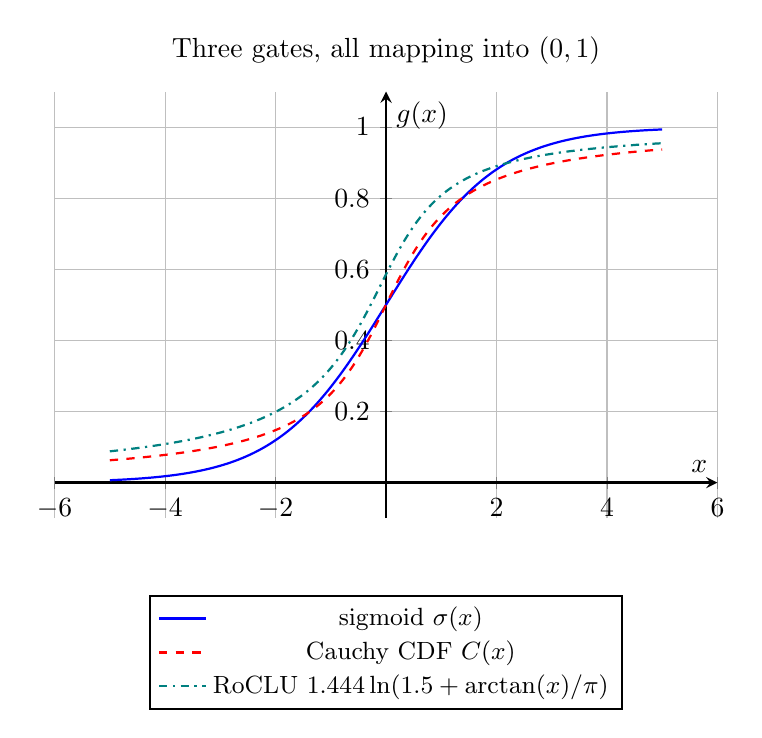
\begin{tikzpicture}
\begin{axis}[
  width=10cm, height=7cm,
  xlabel=$x$, ylabel=$g(x)$,
  title={Three gates, all mapping into $(0,1)$},
  xmin=-6, xmax=6, ymin=-0.1, ymax=1.1,
  axis x line=middle, axis y line=middle,
  grid=major,
  legend style={at={(0.5,-0.18)}, anchor=north, font=\small},
  samples=300, thick,
]
% sigmoid gate
\addplot[blue] {1/(1+exp(-x))};
\addlegendentry{sigmoid $\sigma(x)$}
% Cauchy CDF gate: 1/2 + atan_rad/pi = 1/2 + atan_deg/180
\addplot[red, dashed] {0.5 + atan(x)/180};
\addlegendentry{Cauchy CDF $C(x)$}
% RoCLU gate: 1.444 * ln(1.5 + atan_rad/pi)
\addplot[teal, dashdotted] {1.444*ln(1.5 + atan(x)/180)};
\addlegendentry{RoCLU $1.444\ln(1.5+\arctan(x)/\pi)$}
\end{axis}
\end{tikzpicture}
\end{document}
